% !TEX root = main.tex

\chapter{Path Integrals in the Complex Plane}
\section{Paths}

In real analysis, we often consider the definite integral of a function $f: \R \to \R$ from a real number $a$ to another real number $b$.  Of course, on the real line, there is only one `natural' route from $a$ to $b$, namely, along the real line itself.

\begin{comment}
  There are essentially two ways of interpreting `the integral of $f$ between $a$ and $b$;' either integrating
\begin{center}
from $a$ to $b$, that is, $\int_a^b f(t) \ dt$, or \\
from $b$ to $a$, that is, $\int_b^a f(t)\ dt$.
\end{center}
Of course, these integrals have the same absolute value, but with opposite signs.
\end{comment}

In order to make a sensible definition of integrating `between' two complex numbers $z_1$ and $z_2$, we need to take into account the fact that there are typically many routes from $z_1$ to $z_2$.  An interesting case arises when we consider paths with the same start and end-points.

\begin{figure}[H]
\centering
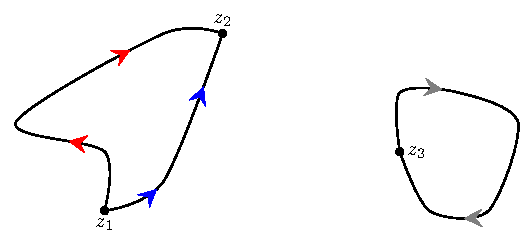
\includegraphics[scale=1]{ch3_path1}
\caption{Some examples of paths between complex numbers.}
\end{figure}

\begin{example}
\label{e:path1}
Consider the line segment $L=[z_1,z_2]$, that is, the straight line segment joining two complex numbers $z_1,z_2 \in \C$.  For an interval $[a,b] \subseteq \R$, define
\[
\gamma : [a,b] \to \C, \quad \gamma (t) = z_1 + \left( \frac{t-a}{b-a} \right) ( z_2 - z_1 ).
\]
Then the line segment $L$ is precisely the range $\gamma \left( [a,b] \right)$ of $\gamma$, with $\gamma (a) = z_1$ and $\gamma (b) = z_2$.

\end{example}

\begin{figure}[H]
\centering
\altgraphics[scale=0.4]{ch3_param1}{ch3_path2}
\caption{The \emph{function} $\gamma:[a,b] \to \C$ describes the \emph{set} $L$, and gives it a direction (i.e. from $\gamma(a)=z_1$ to $\gamma (b)=z_2$).}
\end{figure}

The process of finding $\gamma : [a,b] \to \C$ such that each point on $L$ is of the form $\gamma (t)$, for some $t \in [a,b]$, is called a \emph{parametrisation of $L$}, and we call $t$ the \emph{parameter}.

If we think of $t$ as `time,' then as $t$ increases from $a$ to $b$, $\gamma (t)$ moves from $\gamma (a) = z_1$ to $\gamma (b) = z_2$.  It does so with `velocity'
\begin{align*}
\gamma'(t) &=\ \frac{\text{displacement}}{\text{time}} \\[2ex]
& =\  \frac{\gamma (b) - \gamma (a)}{b-a} = \frac{z_2  - z_1}{b-a}.
\end{align*}
If we think about complex numbers as points or vectors (in $\R^2$), this tells us that $\gamma (t)$ moves in the direction $z_2-z_1$ with constant speed, as you might expect.

We should clarify the definition of the derivative $\gamma'(t)$ of $\gamma(t)$ before we continue.
\begin{definition}
Let $\gamma:[a,b] \to \C$, where $[a,b] \subseteq \R$, be a complex valued function of a real variable.  Then for $t \in [a,b]$, $\gamma$ is said to be differentiable at $t$ if the limit
\[
\rlim{h \to 0}{h \in \R \backslash \set{0}} \frac{\gamma (t+h)-\gamma(t)}{h},
\]
exists.  When it does exist, we denote its value by $\gamma'(t)$, called the \emph{derivative} of $\gamma$ at $t$.
\end{definition}
Note that if $\gamma$ is written in terms of its real and imaginary parts
\[
\gamma(t) = u(t) + i v(t),
\]
where $u,v:[a,b] \to \R$, then we have
\[
\gamma'(t) = u'(t) +i v'(t),
\]
at points $t \in [a,b]$ where these derivatives exist.
%\vspace*{3cm}

\begin{definition}
A \emph{path} is a subset $\Gamma$ of $\C$ for which there is a continuous function $\gamma : [a,b] \to \C$ with
\[
\Gamma = \set{ \gamma (t) : t \in [a,b] }.
\]
The function $\gamma$ is called a \emph{parametrisation} of $\Gamma$, and we call the points $\gamma(a)$ and $\gamma(b)$ the \emph{start-} and \emph{end-points} of $\Gamma$ respectively.
\end{definition}
Note that $\Gamma$ and $\gamma$ are distinct mathematical objects: $\Gamma$ is a set and $\gamma$ is a function.  The function $\gamma$ gives a `direction' to the path $\Gamma$ ; $\Gamma$ is a path \emph{from} $\gamma (a)$ \emph{to} $\gamma(b)$. Thus when we define a path, it is usually necessary to specify a parametrisation, or at least clarify its direction, in order to avoid ambiguity.

There are typically many functions that can be used to paramterise $\Gamma$.  
Having said this, it is perfectly acceptable to define $\Gamma$ by specifying a parametrisation $\gamma$.  Thus if we say ``Consider the path defined by the function $\gamma:[a,b] \to \C$,'' then it is understood that $\Gamma = \set{ \gamma (t) : t \in [a,b] }$.


\begin{example}
\label{e:path2}
For the line segment $L=[z_1,z_2]$, there are many different choices of function $\gamma$ that describe $L$.
\begin{itemize}
\item Taking $a=0$ and $b=1$, $L$ is parametrised by 
\[ \gamma :[0,1] \to \C,\qquad \gamma(t)=z_1+t(z_2-z_1).\]
\begin{blankbox}
Substituting the relevant values of $t$ we see that this path starts at $\gamma(0)=z_1$ and ends at $\gamma(1)=z_2$. Here we have $\gamma'(t)=z_2-z_1$.
\end{blankbox}
\item We could also use the function 
\[
\gamma:[-2,2] \to \C,\ \gamma(t) = z_1 + \left( \frac{t-(-2)}{(2-(-2))} \right) ( z_2-z_1) = \tfrac{1}{2} (z_1+z_2) + t \left( \frac{z_2-z_1}{4} \right).
\]
\begin{blankbox}
This time, $\gamma'(t) = \frac{1}{4} (z_2-z_1)$, which makes sense since it takes 4 units of time for $\gamma(t)$ to move from $z_1$ to $z_2$.
\end{blankbox}
\item Yet another option would be the function 
\[
\gamma: [0,1] \to \C, \qquad \gamma (t) = z_1 + t^2 (z_2-z_1),
\]
\begin{blankbox}
which has non-constant velocity $\gamma'(t) = 2t (z_2-z_1)$.

In all three cases, the \emph{set} $L$ is unchanged, but the \emph{function} $\gamma$ is different.
\end{blankbox}
%\vspace*{8cm}
\end{itemize}
\end{example}



%\vspace*{2cm}
\begin{example}
\label{e:path3}
Fix $R>0$ and consider the function
\[
\gamma:[0,\pi] \to \C, \gamma (t) = R \cos (t) + i R \sin (t).
\]
Let us examine the path described by $\gamma$.
\begin{blankbox}
For all $t$, 
\[ \abs{R \cos(t)+iR \sin (t)} = \sqrt{R^2\cos^2(t)+R^2\sin^2 (t)} = R,
\]
and thus every point $\gamma(t)$ lies on the circle with centre $0$ and radius $R$.  Thus the given path consists of part of this circle.

To determine which part of the circle, we note that $\gamma$
\begin{align*}
& \text{ starts at } \gamma (0) = R\cos(0)+iR\sin(0)=R,\\
& \text{ `visits' }  \gamma \left( \pi /2 \right) = \polar{R}{\pi / 2} = iR \\
& \text{ end at }  \gamma (\pi) = \polar{R}{\pi} = -R.
\end{align*}
Thus $\gamma$ describes the upper semicircle, centre $0$ and radius $R$, traversed in the anticlockwise direction.
%\vspace*{7cm}
\begin{center}
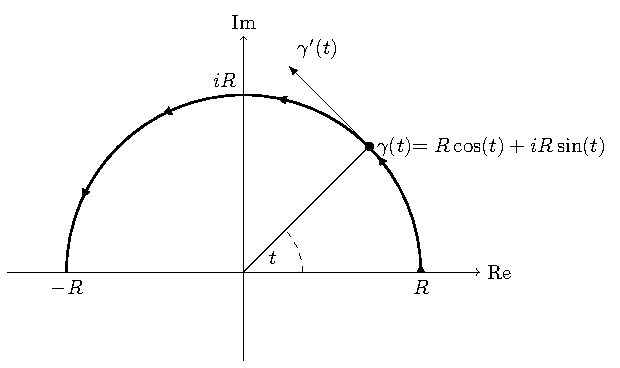
\includegraphics[scale=0.75]{ch3_semicircle0}
\end{center}
%\vspace*{6cm}
The tangent vector to this path at the point $\gamma (t)$ is given by
\begin{align*}
\gamma '(t)& = -R \sin (t) + i R \cos (t) \\
& = i^2 R \sin (t)+iR \cos (t) \\
& = i \gamma (t).
\end{align*}
Thus the tangent vector to the path at the point $\gamma (t)$ is perpendicular to the position vector $\gamma(t)$ (since multiplication by $i$ corresponds to anticlockwise rotation by $\pi/2$).
\end{blankbox}
\end{example}

Note that in examples~\ref{e:path1},~\ref{e:path2} and~\ref{e:path3}, it is necessary to specify both $\gamma(t)$ and the domain of $\gamma$ in order to describe the path completely.  




\begin{definition}
 We say that a parametrisation $\gamma:[a,b] \to \C$ of a path $\Gamma$ is \emph{smooth} if
\begin{enumerate}
\item[(i)] $\gamma$ is differentiable on $[a,b]$,
\item[(ii)] $\gamma'$ is continuous on $[a,b]$, and
\item[(iii)] $\gamma' $ is nonzero on $[a,b]$.
\end{enumerate}
A path $\Gamma$ is called smooth if there exists a smooth parametrisation of $\Gamma$.  
\end{definition}

Informally, a smooth path is one with no corners or sharp turns.  The derivative $\gamma'(t)$, regarded as a vector, is the tangent vector to the path $\Gamma$ at the point $\gamma (t)$.

The paths in Examples~\ref{e:path1}, and~\ref{e:path3} are all smooth.

\begin{definition}
Let $\Gamma$ be a path with smooth parametrisation $\gamma: [a,b] \to \C$.  Then the \emph{reverse} of $\Gamma$ is the path $\tilde{\Gamma}$ consisting of the same set of points as $\Gamma$, but traversed in the opposite direction.  The path $\tilde{\Gamma}$ may be parametrised by the function $\tilde{\gamma} : [a,b] \to \C$ where
\[
\tilde{\gamma} (t) = \gamma (a+b-t) \quad \text{for all } t \in [a,b].
\]
\end{definition}


\begin{blankbox}
Note that if we define the start- and end-points of $\Gamma$ to be
 \[ \gamma (a) = z_1, \quad \gamma (b) = z_2 \] 
 then
\begin{align*}
\tilde{\gamma} (a) & = \gamma (a+b-a) = \gamma (b) = z_2 \\
\tilde{\gamma} (b) & = \gamma (a+b-b) = \gamma (a) = z_1.
\end{align*} 
Thus $\tilde{\Gamma}$ starts at $z_2$ and ends at $z_1$.  Moreover, if $t \in [a,b]$ then $a \leq a+b-t \leq b$, and so $\tilde{\gamma} (t)$ describes a point on the original path $\Gamma$ (i.e. $\tilde{\Gamma}$ is the same set as $\Gamma$).

The tangent vector is given by
\[
\tilde{\gamma} ' (t) = \frac{d}{dt} \gamma (a+b-t) = \gamma'(a+b-t) \frac{d}{dt}(a+b-t) = - \gamma'(a+b-t).
\]
In other words, at any point $z = \tilde{\gamma} (t) = \gamma (a+b-t)$ on the path $\Gamma$, the tangent vector to this path at $z$, when travelling in the reverse direction, points in the opposite direction to the tangent vector obtained when travelling in the original direction, as expected.
\end{blankbox}

\begin{example}
Let us find the reverse of the paths considered in Examples~\ref{e:path2} and~\ref{e:path3}.
\end{example}
\begin{solution}
\begin{itemize}
\item $L=[z_1, z_2 ] $, parametrised by $\gamma:[0,1] \to \C$, $\gamma (t) = z_1 + t ( z_2 - z_1 )$.
It is clear that the reverse of $L$ is the line segment $\tilde{L}=[z_2,z_1]$, i.e. the same line segment taken from $z_2$ to $z_1$.  We may parametrise $\tilde{L}$ with the function $\tilde{\gamma}:[0,1] \to \C$, where
\begin{align*}
\tilde{\gamma} (t) & = \gamma (0+1-t ) \\
& = z_1 + (1-t)(z_2-z_1) \\
& = z_2+t(z_1-z_2).
\end{align*}
On examining the equation for $\tilde{\gamma} (t)$, it is clear that this function describes the path that starts at $z_2$ and travels in the direction $(z_1-z_2)$.
\item  $\Gamma$ the semicircle parametrised by $\gamma:[0,\pi] \to \C$ , $\gamma (t) = R \cos (t) + i R \sin (t)$. 

In this case $\tilde{\Gamma}$ is the clockwise semicircular arc from $-R$ to $R$ via $iR$.  We may parametrise $\tilde{\Gamma}$ using $\tilde{\gamma}:[0,\pi] \to \C$, where
\begin{align*}
\tilde{\gamma} (t) & = \gamma ( \pi-t) \\
& = R \cos ( \pi-t)+iR \sin (\pi-t) \\
& = -R \cos (t) + i R \sin (t).
\end{align*}
Note that $\tilde{\gamma} (t)$ is $\gamma (t)$ reflected through the imaginary axis; and thus the path $\tilde{\Gamma}$ is the reflection of the path $\Gamma$ in the imaginary axis.
%\vspace*{9cm}

\end{itemize}
\end{solution}

We shall often need to consider the paths that we obtain from joining smooth paths together.  Note that the resulting path may fail to be smooth, e.g., if there is a `corner' at the point where they meet.

Suppose we have two or more (smooth) paths $\Gamma_1,\ \Gamma_2$ etc., parametrised by $\gamma_1:[a_1,b_1] \to \C$ and $\gamma_2:[a_2,b_2] \to \C$, and suppose that the end-point of $\Gamma_1$ is the same as the start-point of $\Gamma_2$, i.e. $\gamma_1(b_1)=\gamma_2(a_2)$.

The curve obtained from $\Gamma_1 \cup \Gamma_2 $ certainly looks like a path, but how do we make this precise?  In other words, can we describe this curve as the image of some continuous $\gamma: [a,b] \to \C$?
\begin{figure}[H]
\centering
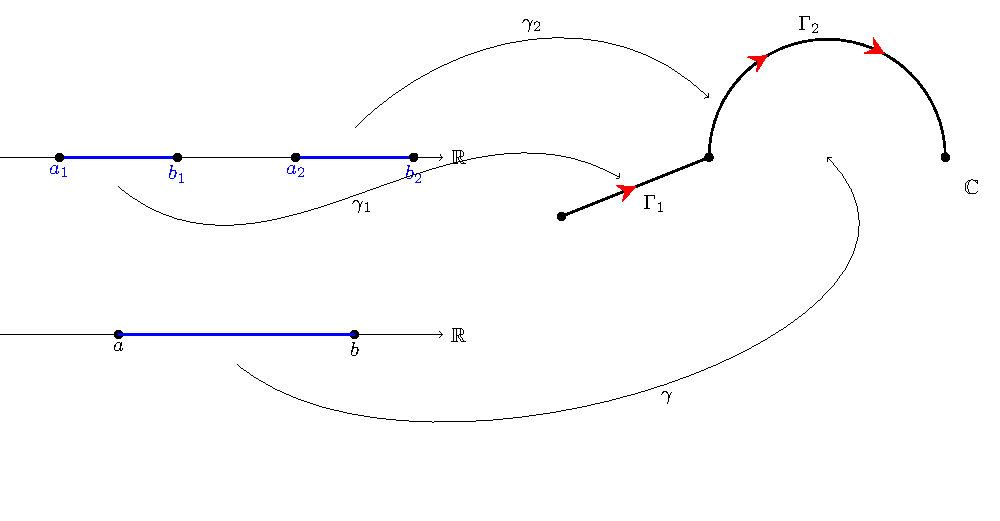
\includegraphics[scale=0.75]{ch3_join4}
\caption{We have two functions $\gamma_1:[a_1,b_1] \to \C$ and $\gamma_2:[a_2,b_2] \to \C$ parameterising $\Gamma_1$ and $\Gamma_2$ respectively.  We want a single continuous function $\gamma:[a,b] \to \C$ parameterising $\Gamma_1 \cup \Gamma_2$}.
\end{figure}
\begin{blankbox}
To do this, we first move $[a_2,b_2]$ to an interval from $b_1$ and then reparametrise $\Gamma_2$.  For $t \in \R$, let $\alpha(t)=  t-(a_2-b_1)$, so that $\alpha$ maps $[a_2,b_2]$ bijectively to $[b_1,b_1+b_2-a_2]$.
\begin{figure}[H]
\centering
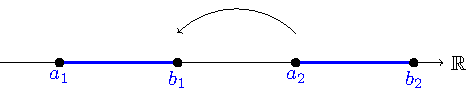
\includegraphics[scale=1]{ch3_join5}
\end{figure}
%\vspace*{5cm}
Now, parametrise $\Gamma_2$ using the function $\gamma_{1+2}:[b_1,b_1+b_2-a_2] \to \C$, where
\[
\gamma_{1+2} (t) = \gamma_2 ( \alpha^{-1} (t) ) = \gamma_2 (t+a_2-b_1)
\]
for all $t \in [b_1,b_1+b_2-a_2]$.
\end{blankbox}
\begin{definition}
Suppose that $\Gamma_1$ and $\Gamma_2$ are two paths parametrised by $\gamma_1:[a_1,b_1] \to \C$ and $\gamma_2:[a_2,b_2] \to \C$ respectively, such that $\gamma_1(b_1) = \gamma_2 (a_2)$.  Then we define the \emph{join} of $\Gamma_1$ and $\Gamma_2$ to be the path $\Gamma_1+\Gamma_2$ parametrised by $\gamma_{1+2}:[a_1,b_1+b_2-a_2] \to \C$, where
\[
\gamma_{1+2} (t) = \begin{cases}
\gamma_1 (t) & t \in [a_1,b_1] \\
\gamma_2 (t-b_1+a_2) & t \in [b_1,b_1+b_2-a_2].
\end{cases}
\]
\end{definition}


If we have another path $\Gamma_3$ we can join $\Gamma_3$ to $\Gamma_1+\Gamma_2$ to get $\Gamma_1+\Gamma_2+\Gamma_3$ and so on.

\begin{definition}
A \emph{contour} is a path which is the join of finitely many smooth paths.
\end{definition}

\begin{figure}[H]
\centering
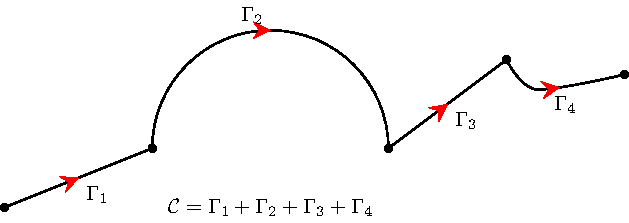
\includegraphics[scale=1]{ch3_contour}
\caption{A contour $\mathcal{C}$ constructed from the join of smooth paths $\Gamma_1,\Gamma_2,\Gamma_3,\Gamma_4$.  Note that $\mathcal{C}$, considered as a path in its own right, need not be smooth.}
\end{figure}


\begin{definition}
Let $\Gamma$ be a smooth path parametrised by $\gamma:[a,b] \to \C$.  Then the \emph{length} $\ell ( \Gamma)$ of $\Gamma$ is defined to be
\[
\ell ( \Gamma ) : = \int_a^b \abs{ \gamma '(t) } \ dt.
\]
For a contour $\mathcal{C} = \Gamma_1+\Gamma_2 + \ldots + \Gamma_n$, where $\Gamma_1,\Gamma_2, \ldots , \Gamma_n$ are smooth, we define the \emph{length} $\ell ( \mathcal{C} )$ of $\mathcal{C}$ to be
\[
\ell ( \mathcal{C} ) = \ell ( \Gamma_1 ) + \ell ( \Gamma_2 ) + \ldots + \ell ( \Gamma_n).
\]
\end{definition}


\begin{example}
Let us compute the length of the line segment $L=[0,3+4i]$ using the parametrisation $\gamma: [0,1] \to \C$ where
\[
\gamma (t) = (3+4i)t, \quad t \in [0,1].
\]
\end{example}
\begin{solution}
We have $\gamma'(t)=3+4i$, with modulus $\abs{\gamma'(t)} = \abs{3+4i}=5$ for all $t$.  Hence
\[
\ell (L) = \int_0^1 \abs{\gamma'(t)} \ dt = \int_0^1 5\ dt = 5,
\]
which is what we would expect given the geometry of this line segment.
\begin{center}
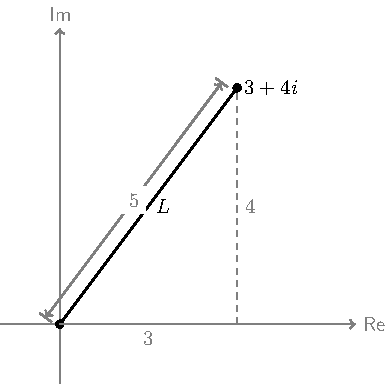
\includegraphics[scale=0.8]{ch3_path6}
\end{center}
%\vspace*{3cm}
\end{solution}
\begin{example}

Now we shall compute the length of the semicircular path $\Gamma$ described by $\gamma : [0,\pi] \to \C$
\[
\gamma (t) = R \cos (t) + i R \sin (t), \quad t \in [0,\pi].
\]
\end{example}
\begin{solution}
We have shown already that for all $t\in [0,\pi]$, $\gamma'(t)=i\gamma(t)$, and so
\[
\abs{\gamma'(t)} = \abs{i \gamma (t)} = \abs{i} \abs{ R \cos(t)+iR\sin(t)} = R
\]
for all such $t$.  It follows that
\[
\ell ( \Gamma ) = \int_0^{\pi} R\ dt = \pi R,
\]
which is again what we would expect for a semicircle with radius $R$.
%\vspace*{8cm}

\end{solution}

\section{The Integral along a path in $\C$}
In this section we will define the integral of a complex function along a smooth path $\Gamma$.  We first recall the following results about integrals of real functions from Foundations.
\begin{theorem}
\label{t:realint}
Let $f,g:[a,b] \to \R$ be two \emph{continuous} real valued functions defined on some interval $[a,b] \subset \R$.  Then the integrals $\int_a^b f(t)\ dt$ and $\int_a^b g(t)\ dt$ both exist and satisfy the following properties:
\begin{enumerate}
\item[(i)] (Linearity) For any $c \in \R$ we have
\[
\int_a^b \left( cf(t) +  g(t) \right)\ dt = c\int_a^b f(t)\ dt +  \int_a^b g(t)\ dt.
\]
\item[(ii)] (Fundamental Theorem of Calculus) If $F:[a,b]$ is an antiderivative for $f$ on $[a,b]$ (that is, $F'(t) = f(t)$ for all $t \in [a,b]$), then 
\[
\int_a^b f(t)\ dt = F(b) - F(a),
\]
\item[(iii)] (Monotonicity) If $f(t) \leq g(t)$ for all $t \in [a,b]$ then
\[
\int_a^b f(t)\ dt \leq \int_a^b g(t)\ dt.
\]
\end{enumerate}
\end{theorem}
We shall frequently use the results of Theorem~\ref{t:realint} without reference.

Now let us define the integral of a complex-valued function of a real variable, $g:[a,b] \to \C$ defined on some interval $[a,b] \subset \R$.

\begin{definition}
\label{d:realint}
Let $g:[a,b] \to \C$ be a complex valued function defined on the (real) interval $[a,b]$, and assume that the real and imaginary parts $\Re (g)$ and $\Im (g)$ are both continuous.  Then we define the integral of $g$ from $a$ to $b$ via
\[
\int_a^b g(t)\ dt = \int_a^b \Re (g) (t)\ dt + i \int_a^b \Im (g) (t)\ dt.
\]
\end{definition}
Note that the functions $\Re (g)$ and $\Im (g)$ are both real-valued and continuous, and so we have defined the integral of $g$ in terms of integrals of real functions.  So for example,
\[
\int_0^1 t+i2t\ dt = \int_0^1 t\ dt +i \int_0^1 2t\ dt = \left[ \frac{t^2}{2} \right]_0^1 + i \left[ 2 \frac{t^2}{2} \right]_0^1
= \frac{1}{2}+i.\]


Using the definition of the integral of a complex-valued function of a real variable, together with Theorem~\ref{t:realint}, the results of Theorem~\ref{t:cint1} follow easily.

\begin{theorem}
\label{t:cint1}
Let $f,g:[a,b] \to \C$ be complex valued functions of a real variable defined on the interval $[a,b] \subset \R$, and assume that the real and imaginary parts of both $f$ and $g$ are all continuous.  Then the integrals $\int_a^b f(t)\ dt$ and $\int_a^b g(t)\ dt$ both exist and satisfy the following properties:
\begin{enumerate}
\item[(i)] (Linearity) For any $\alpha \in \C$ we have
\[
\int_a^b \left( \alpha f(t) +  g(t) \right)\ dt = \alpha \int_a^b f(t)\ dt +  \int_a^b g(t)\ dt.
\]
\item[(ii)] (Fundamental Theorem of Calculus) If $F:[a,b] \to \C$ is an antiderivative for $f$ on $[a,b]$ (that is, $F'(t) = f(t)$ for all $t \in [a,b]$), then 
\[
\int_a^b f(t)\ dt = F(b) - F(a).
\]
\end{enumerate}
\end{theorem}
Note that there is no way to extend Theorem~\ref{t:realint}(iii) to complex valued functions, as there is no sensible way to interpret the expression $\alpha \leq \beta $ for $\alpha, \beta \in \C$.


\begin{definition}
Let $U \subseteq \C$ be open, $f:U \to \C$ a continuous function and let $\Gamma$ be a smooth path contained in $U$, parametrised by $\gamma :[a,b] \to \C$.  Then the \emph{integral of $f$ along $\gamma$}, which we write as 
\[
\int_{\Gamma} f,
\]
is defined via
\begin{equation}
\label{e:pathint}
\int_{\Gamma} f = \int_a^b f \left( \gamma(t) \right) \gamma ' (t)\ dt.
\end{equation}
\end{definition}

\begin{note}
\begin{enumerate}
\item[(i)] The composition $f \left( \gamma (t) \right)$ is a complex valued function of a real variable, hence so is $f \left( \gamma (t) \right) \gamma '(t)$.  It follows that the integral
\[
\int_a^b f \left( \gamma(t) \right) \gamma ' (t)\ dt
\]
on the right hand side of~\eqref{e:pathint} is of the type defined in Definition~\ref{d:realint}.
\item[(ii)] It is sometimes convenient to write
\[
\int_{\Gamma} f \text{ as } \int_{\Gamma} f(z)\ dz \text{ or } \int_{\Gamma} f ( \zeta ) \ d \zeta.
\]
\item[(iii)] The value of the integral depends on both the function $f$ and the path $\Gamma$.  It looks like it should also depend on our choice of parametrisation $\gamma$, but this is not the case.
\end{enumerate}
\end{note}


\begin{example}
\label{e:3paths}
Fix $\alpha$ and $\beta \in \C$ and let $f:\C \to \C$ be defined by
\[
f(z) = \alpha z + \beta \conj{z}.
\]
Let us compute the value of $\int_{\Gamma} f$ along each of the three paths
\begin{align*}
 \Gamma_1&=[0,2]\\
 \Gamma_2&=[2,2+2i] \\
 \Gamma_3 &=[2+2i,0].
\end{align*}
\end{example}
\begin{solution}
Following the method of Example~\ref{e:path2}, parametrise each $\Gamma_j$ by the function $\gamma_j:[0,1] \to \C$, where
\begin{align*}
\gamma_1 (t) & = 2t \\
\gamma_2 (t) &= 2+i 2t \\
\gamma_3 (t) & = (1-t)(2+2i)
\end{align*}
for $t \in [0,1]$.

For the path $\Gamma_1$, we have
\[
f (\gamma_1 (t) ) = \alpha (2t)+\beta (\conj{2t}) = (\alpha+\beta)(2t) \text{ and } \gamma_1'(t) = 2
\]
for all $t \in [0,1]$.  Thus 
\begin{align*}
\int_{\Gamma_1} f &= \int_0^1 f( \gamma_1(t)) \gamma_1'(t)\ dt \\
&= \int_0^1 (\alpha+\beta)(2t)(2)\ dt \\
& = 4(\alpha+\beta) \int_0^1 t\ dt = 2(\alpha+\beta). 
\end{align*}
For $\Gamma_2$, we have
\begin{align*}
f ( \gamma_2(t)) & = \alpha (2+i2t)+\beta ( \conj{2+i2t} ) \\
& = \alpha (2+i2t)+\beta (2-2it) \\
\shortintertext{ and }
\gamma_2'(t) &= 2i. \\
\shortintertext{ hence }
f ( \gamma_2(t) ) \gamma_2' (t) & = \alpha (2+i2t)+\beta (2-2it) 2i \\
& = -4(\alpha-\beta)t + 4i (\alpha+\beta),
\shortintertext{ and so the required path integral is }
\int_{\Gamma_2} f& = \int_0^1 \left[-4(\alpha-\beta)t + 4i (\alpha+\beta)\right]\ dt \\
& = \left( -4(\alpha-\beta) \int_0^1 t\ dt \right) +i \left( 4(\alpha+\beta) \int_0^1 1\ dt \right) \\
& = -2(\alpha-\beta)+4i(\alpha+\beta).
\end{align*}
Finally, we have
\begin{align*}
f ( \gamma_3 (t) ) & = 2(\alpha+\beta)(1-t)+i 2 (\alpha-\beta)(1-t) \\
\gamma_3'(t) & = -2-2i \\
\shortintertext{ so that }
f ( \gamma_3 (t)) \gamma_3'(t) & = \left[ \alpha (2+2i)+\beta(2-2i) \right] (-2-2i)(1-t) \\
\shortintertext{ giving }
\int_{\Gamma_3} f & = \left[ \alpha (2+2i)+\beta(2-2i) \right] (-2-2i) \int_0^1 (1-t)\ dt \\
& = -4\beta-4\alpha i.
\end{align*}
\end{solution}

\begin{example}
 Find
\[
\int_{\Gamma} f,
\]
where $f$ is the complex function $f(z)=\conj{z}$ and $\Gamma$ is the semicircular path joining $1$ and $-1$ defined by $\gamma : [0, \pi] \to \C$,  $\gamma(t)=\cos(t) + i \sin (t)$.
\end{example}
\begin{solution}
%\begin{framed}
%\vspace{10cm}
%\end{framed}
Here we have
\[
f(\gamma(t)) = \conj{\cos(t)+i\sin(t)} = \cos(t)-i \sin(t),
\]
and $\gamma'(t) = -\sin(t)+i \cos (t)$, so that
\begin{align*}
f(\gamma(t))\gamma '(t) &=  \left(-\sin(t)+i \cos (t) \right) \left( \cos(t)-i \sin(t) \right)\\
& = -\cos(t)\sin(t)+\sin(t)\cos(t) +i \left[ (-\sin(t))(-\sin(t))+\cos(t)\cos(t) \right] \\
& = i.
\end{align*}
Hence
\[
\int_{\Gamma} \conj{z}\ dz = \int_0^{\pi} i\ dt = \pi i.
\]
\end{solution}
We now extend the definition of the integral along a smooth path to the integral along a contour $\mathcal{C}$ which is the join of a finite number of smooth paths $\Gamma_1,\Gamma_2, \ldots , \Gamma_n$ as follows:
\[
\int_{\mathcal{C}} f = \int_{\Gamma_1} f + \int_{\Gamma_2} f + \ldots + \int_{\Gamma_n} f
\]
\begin{example}
\label{e:triangle}
Compute the value of $\int_{\mathcal{C}} f$ where $f=\alpha z + \beta \conj{z}$ and $\mathcal{C}=\Gamma_1 + \Gamma_2 + \Gamma_3$ from Example~\ref{e:3paths}.
\end{example}

\begin{solution}
\begin{center}
\begin{tikzpicture}
\draw[thick,gray,->] (-2,0) -- (3,0) ;
\draw[thick,gray,->] (0,-1) -- (0,3) ;
\draw[thick] (0,0) -- node[midway,below,font=\footnotesize]{$\Gamma_1$} (2,0) node[below,font=\footnotesize]{$2$};
\draw[thick] (2,0) -- node[midway,right,font=\footnotesize]{$\Gamma_2$} (2,2) node[right,font=\footnotesize]{$2+2i$};
\draw[thick] (2,2) -- node[midway,left,font=\footnotesize]{$\Gamma_3$} (0,0);
\end{tikzpicture}
\end{center}
Here we have
\begin{align*}
\int_{\mathcal{C}} f & = \int_{\Gamma_1} f + \int_{\Gamma_2} f + \int_{\Gamma_3} f \\
& = 2(\alpha+\beta)-2(\alpha-\beta)+4i(\alpha+\beta)\\
&-4\beta-4\alpha i \\
& = i 4 \beta.
\end{align*}

Note that the function $f(z) =\alpha z + \beta \conj{z}$ is not differentiable anywhere in $\C$ unless $\beta = 0$.  Moreover, if $\beta = 0$ then $f(z)=\alpha z$ is holomorphic on $\C$ and $\int_{\mathcal{C}} f = 0$ for the contour $\mathcal{C}=\Gamma_1+\Gamma_2+\Gamma_3$ in the preceding example, while $\int_{\mathcal{C}} f \neq 0$ when $\beta \neq 0$.  This is not a coincidence, as we shall see in subsequent sections.
\end{solution}
\section{The Fundamental Theorem of Complex Calculus}
\begin{definition}
A set $S \subseteq \C$ is \emph{connected} if given any pair of points $z_1,z_2 \in S$, there is a contour contained in $S$ that starts at $z_1$ and ends at $z_2$. A \emph{region} $\mathcal{R}$ is a non-empty, open, connected subset of $\C$.
\end{definition}
\begin{figure}[H]
\centering
\blankgraphics[scale=0.5]{ch3_connected} \qquad \blankgraphics[scale=0.5]{ch3_notconnected}
\end{figure}
\begin{definition}
Let $\mathcal{R}$ be a region and $f:\mathcal{R} \to \C$ a function defined on $\mathcal{R}$.  A function $F:\mathcal{R} \to \C$ is called an \emph{antiderivative for $f$ on $\mathcal{R}$} if
\begin{enumerate}
\item[(i)] $F$ is holomorphic on $\mathcal{R}$ and
\item[(ii)] $F'(z)=f(z)$ for all $z \in \mathcal{R}$.
\end{enumerate}
\end{definition}
\begin{example}
Find antiderivatives for the functions
\begin{enumerate}
\item[(i)] $f(z)=\alpha z + \beta$ (where $\alpha, \beta \in \C$ are fixed) on the region $\C$.
\item[(ii)] $f(z) = \dfrac{1}{(1+iz)^2}$ on the region $\C \backslash \set{i}$. 
\end{enumerate}
\end{example}
\begin{solution}
\begin{enumerate}
\item[(i)] The function $F$ defined by $F(z) = \frac{\alpha}{2} z^2+\beta z$ is an antiderivative for $f$ on $\C$, as $F$ is holomorphic on $\C$ with $F'(z)=f(z)$ for all $z$.
\item[(ii)] The function $F:\C \backslash \set{i} \to \C$ defined by
\[
F(z)=\frac{i}{1+iz}
\]
is an antiderivative for $f$ on $\C \backslash \set{i}$ by the quotient rule.
\end{enumerate}
\end{solution}
\begin{question}
Does the function $f(z) = \conj{z}$ have an antiderivative on $\C$?  We will answer this question shortly.
\end{question}
%\vspace*{2cm}
We know already that $f(z)=\conj{z}$ cannot be the antiderivative of any function $g:\C \to \C$ as $f$ is not differentiable anywhere.
\begin{theorem}[Fundamental Theorem of Complex Calculus]
\label{t:ftc}
Let $f$ be continuous on a region $\mathcal{R}$ suppose that $F$ is an antiderivative for $f$ on $\mathcal{R}$.  If $\mathcal{C}$ is a contour contained in $\mathcal{R}$, then we have
\[
\int_{\mathcal{C}} f = F( z_2)-F(z_1)
\]
where $z_1$ and $z_2$ are the start- and end-points of $\mathcal{C}$ respectively.
\end{theorem}
\begin{proof}

Let us first consider the case where $\mathcal{C}$ consists of a single smooth path $\Gamma$, parametrised by $\gamma:[a,b] \to \C$.  Since $F$ is an antiderivative for $f$ on $\mathcal{R}$ and $\gamma$ is smooth, the Chain Rule gives
\[
\frac{d}{dt} \left[ F( \gamma(t)) \right] = F'(\gamma(t))\gamma'(t) = f(\gamma(t))\gamma ' (t).
\]
Hence
\begin{align*}
\int_{\Gamma} f & = \int_a^b f(\gamma(t)) \gamma' (t)\ dt & \\
& = \int_a^b \frac{d}{dt} \left[ F( \gamma (t) ) \right]\ dt & \\
& = F ( \gamma (b) ) - F ( \gamma (a) ) & \text{ by Theorem~\ref{t:cint1}(ii)} \\
& = F(z_2)-F(z_1).
\end{align*}


%\vspace*{14cm}

Now, if $\mathcal{C}$ is the join of $n$ smooth paths $\mathcal{C} = \Gamma_1+\ldots + \Gamma_n$, let $w_{j-1}$ and $w_j$ denote the start- and end-points of $\Gamma_j$ respectively, so that $w_0=z_1$ and $w_n=z_2$.  Then

\begin{align*}
\int_{\mathcal{C}} f & = \int_{\Gamma_1} f + \int_{\Gamma_2} f + \ldots + \int_{\Gamma_n} f \\
& = \left( F(w_1)-F(w_0) \right) + \left( F(w_2)-F(w_1) \right) + \ldots + \left( F(w_n)-F(w_{n-1}) \right) \\
& = F(w_n)-F(w_0) = F(z_2)-F(z_1).
\end{align*}


\end{proof}
The Fundamental Theorem of Complex Calculus tells us that if an antiderivative $F$ for $f$ on $\mathcal{R}$ is known, then a potentially complicated contour integral $\int_{\mathcal{C}} f$ may be evaluated by simply computing the values of $F(z_1)$ and $F(z_2)$.

\begin{example}
\label{e:2paths}
Let $\alpha \in \C$ be fixed and let $f(z)=\alpha z$ for all $z \in \C$.  We shall evaluate $\int_{\mathcal{C}} f$ along the contour $\mathcal{C}=\Gamma_1 + \Gamma_2$ where $\Gamma_1=[0,2]$ and $\Gamma_2 = [2,2+2i]$ using Theorem~\ref{t:ftc}.
\end{example}
\begin{solution}
The function $F$ defined by $F(z)=\frac{\alpha}{2} z^2$ is an antiderivative for $f$ on $\C$.
  The start- and end-points of $\mathcal{C}$ are $0$ and $2+2i$ respectively.  Hence by the Fundamental Theorem of Complex Calculus,
\begin{align*}
\int_{\mathcal{C}} f &= F(2+2i)-F(0) \\
& = \frac{\alpha (2+2i)^2}{2} - 0 \\
& = i 4 \alpha.
\end{align*}
\end{solution}

\begin{example}
With $f,\Gamma_1$ and $\Gamma_2$ as in Example~\ref{e:2paths} and let $\Gamma_3 = [2+2i,0]$.  We will calculate $\int_{\mathcal{C}} f$ where $\mathcal{C}=\Gamma_1+\Gamma_2+\Gamma_3$.
\end{example}
\begin{solution}
This time $\mathcal{C}$ starts and ends at $0$, so that
\[
\int_{\mathcal{C}} f = F(0) - F(0) = 0.
\]
\end{solution}

\begin{example}
Let $\Gamma_1$ be the path consisting of the arc of the circle of radius $2$, centre $0$, traversed in the anticlockwise direction from $2$ to $-2$ and let $\Gamma_2$ be the line segment $[-2,-i]$.  Calculate
\[
\int_{\mathcal{C}} f,
\]
where $f(z) = \dfrac{1}{(1+iz)^2}$ and $\mathcal{C} = \Gamma_1+ \Gamma_2$.
\end{example}
\begin{solution}
\begin{center}
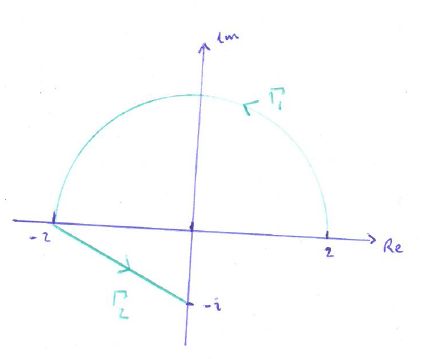
\includegraphics[scale=0.5]{ch3_ftc2}
\end{center}
The contour $\mathcal{C}$ is contained in the region $\C \backslash \set{i}$, and $F(z) = \frac{i}{(1+iz)}$ is an antiderivative for $f$ on this region.  Since $\mathcal{C}$ starts at $2$ and ends at $-i$, we have
\begin{align*}
\int_{\mathcal{C}} f & = F(-i)-F(2) \\
& = \frac{i}{2} - \frac{i}{1+2i} \\
& = - \frac{2}{5} +i \frac{3}{10}.
\end{align*}
\end{solution}
\begin{theorem}[Contour Independence]
\label{t:contint}
Let $f$ be continuous on $\mathcal{R}$ and let $F$ be an antiderivative for $f$ on $\mathcal{R}$.  If $\mathcal{C}_1$ and $\mathcal{C}_2$ are two contours inside $\mathcal{R}$ with the same start- and end-points, we have
\[
\int_{\mathcal{C}_1} f = \int_{\mathcal{C}_2} f.
\]
\end{theorem}
\begin{proof}
Let $z_1$ be common the start-point of both $\mathcal{C}_1$ and $\mathcal{C}_2$, and $z_2$ the end-point.  Then by Theorem~\ref{t:ftc},
\[
\int_{\mathcal{C}_1} f = F(z_2)-F(z_1) = \int_{\mathcal{C}_2} f.
\]
\end{proof}
One application of Theorem~\ref{t:contint} is that it allows us to replace a potentially complicated contour integral along $\mathcal{C}_1$ with an easier one alone $\mathcal{C}_2$.

\begin{definition}
A contour $\mathcal{C}$ is called a \emph{closed contour} if its end point is the same as its start point.
\end{definition}
\begin{theorem}[Antiderivatives and Closed Contours]
\label{t:closed}
Let $f$ be continuous on $\mathcal{R}$ and let $F$ be an antiderivative for $f$ on $\mathcal{R}$.  If $\mathcal{C}$ is any closed contour inside $\mathcal{R}$ then
\[
\int_{\mathcal{C}} f = 0.
\]
\end{theorem}
\begin{proof}
This time $\mathcal{C}$ has the same start- and end-point $z_1$.  Hence
\[
\int_{\mathcal{C}} f = F(z_1)-F(z_1) = 0.
\]
\end{proof}


\begin{question}
Now, do we know whether or not $f(z)=\conj{z}$ has an antiderivative on $\C$?  Does Example~\ref{e:triangle} tell you anything?
\end{question}
%\vspace*{5cm}
\begin{answer}
 The function $f(z) = \conj{z}$ is a special case of the function considered in Example~\ref{e:triangle}, with $\alpha =0$ and $\beta =1$.  If $\mathcal{C}$ is the closed triangular contour of that example, then we have seen that
\[
\int_{\mathcal{C}}  \conj{z}\ dz = 4i \neq 0.
\]
Thus as a consequence of Theorem~\ref{t:closed}, we see that $f(z)=\conj{z}$ cannot have an antidervative on $\C$.
\end{answer}
\begin{theorem}[Zero Derivative Theorem]
Let $F$ be holomorphic on a region $\mathcal{R}$ and suppose that $F'(z)=0$ for all $z \in \mathcal{R}$.  Then $F$ is constant on $\mathcal{R}$.
\end{theorem}
\begin{proof}
Let $z_1,z_2 \in \mathcal{R}$.  We will show that $F(z_1)=F(z_2)$.

Since $\mathcal{R}$ is connected there is a contour $\mathcal{C}$ in $\mathcal{R}$ that starts at $z_1$ and ends at $z_2$.  Hence by Theorem~\ref{t:ftc},
\[
F(z_2)-F(z_1) = \int_{\mathcal{C}} F'(z)\ dz = \int_{\mathcal{C}} 0\ dz = 0.
\]
In other words $F(z_1)=F(z_2)$.  Since this is true for all $z_1,z_2 \in \mathcal{R}$, $F$ must be constant on $\mathcal{R}$.
\end{proof}

%\vspace*{12cm}